%
% ---------------------------------------------------
%
% Proyecto Final de Carrera: EMIR
% Autor: Pedro Hernández Martín <alu3679@etsii.ull.es>
% Capítulo: Estado del arte
% Fichero: Cap2_estado_del_arte.tex
%
% ----------------------------------------------------
%

\chapter{Algoritmos} \label{chap:algorithm}

El objetivo del \CSUO{} es cubrir (abarcar) todos los objetos 
presentes en el campo observado, con el menor
número de apuntados posible. Para resolver este problema se plantearon varios
posibles frentes de actuación, explicados brevemente a continuación, y
exhaustivamente al final del Capítulo, donde se detalla el algoritmo
utilizado.

\section{Clustering} \label{sec:clustering}

El primer enfoque que se exploró fue el de utilizar la densidad que presentan los
objetos en su distribución espacial, de forma que se actúe primero sobre zonas donde existe un
mayor número de puntos. Para diferenciar las zonas en la que se agrupan los
objetos se ha utilizado el algorimo DBScan.
Para ello se partió del código \cite{Web:GITDBS} adaptándolo y traduciéndolo a C++.

El Algoritmo \ref{alg:pseudo-dbscan} muestra un pseudo-código para el DBScan.

\begin{algorithm}[H]
DBSCAN($D$, $eps$, $MinPts$) \{

   $C = 0$

   \For{(cada punto $P$ no visitado en el cjto de datos $D$)} {

      marcar $P$ como visitado

      $NeighborPts =$ regionQuery($P$, $eps$)

      \eIf{(sizeof($NeighborPts$) $< MinPts$)} { marcar $P$ como $RUIDO$ } {

         $C =$ siguiente cluster

         expandCluster($P$, $NeighborPts$, $C$, $eps$, $MinPts$)
      }
    }
\}

expandCluster($P$, $NeighborPts$, $C$, $eps$, $MinPts$) \{

  añadir $P$ al cluster $C$

  \For{(cada punto $P'$ en $NeighborPts$)} {% 

     \If{($P'$ no visited)} {%

       marcar $P'$ como visitado

       $NeighborPts' = $regionQuery($P'$, $eps$)

       \If{(sizeof($NeighborPts'$) $>= MinPts$)} {%

         $NeighborPts = NeighborPts$ unido a $NeighborPts'$
       }
     }

     \If{($P'$ todavía no es miembro de algún cluster)} {%

       añadir $P'$ al cluster $C$
     }
   }
\}

regionQuery($P$, $eps$) \{

   return todos los puntos vecinos de $P'$ (incluyendo $P$)
   %return all points within $P'$s eps-neighborhood (including $P$)
\}

\caption{Pseudo-código del algoritmo DBSCAN}
\label{alg:pseudo-dbscan}
\end{algorithm}

Los clusters obtenidos dependen de dos parámetros, \textit{eps} y \textit{Min\_Pts} que indican respectivamente la
distancia que se permite entre puntos y el número mínimo de objetos requeridos
para formar un cluster. 
Para obtener buenos resultados es necesario un
conocimiento profundo del problema de entrada, puesto que se deben variar los
parámetros según la distribución de los objetos del mismo. Este procesado
resulta costoso y poco rentable, puesto que por lo general este tipo de
algoritmos presenta pobres resultados en problemas con distribuciones espaciales
homogéneas.

%%%%%%%%%%%%%%%%%%% Fig. %%%%%%%%%%%%%%%%%%%%%%%%%%%%%%%%%%%
\begin{figure}[!htb]
\centering
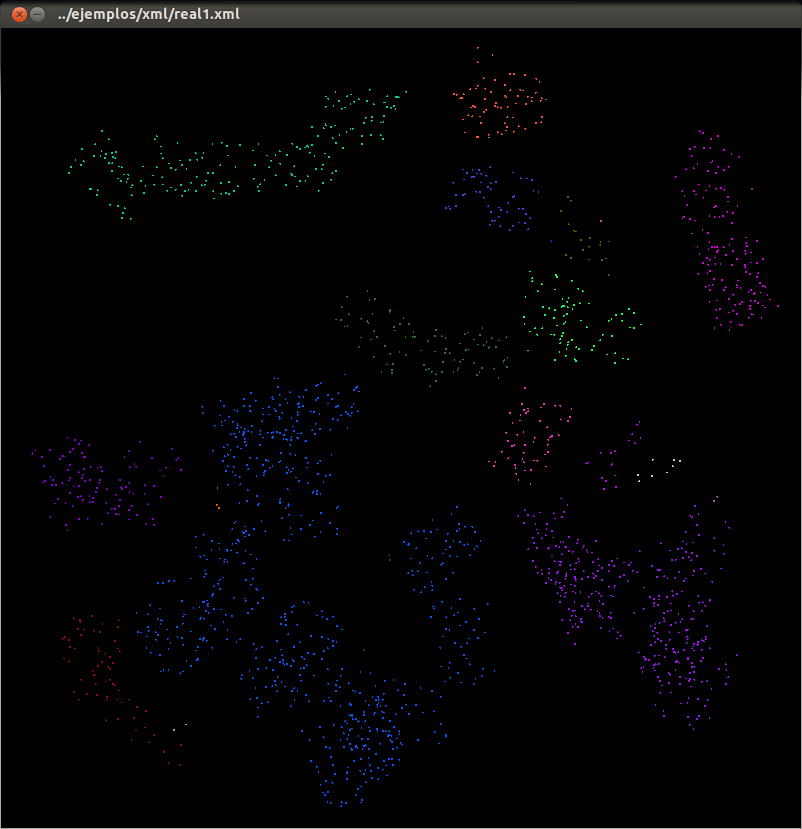
\includegraphics[width=0.7\linewidth]{dbscan-e86-m4}
\caption{Resultado de aplicar DBSCAN al \texttt{real1.xml}}
\label{fig:dbscan-e86-m4}
\end{figure}
%%%%%%%%%%%%%%%%%%%%%%%%%%%%%%%%%%%%%%%%%%%%%%%%%%%%%%%%%%%%%%

En la Figura \ref{fig:dbscan-e86-m4} se puede observar el resultado del
algoritmo aplicado al ejemplo \texttt{real1.xml} (cuya representación se puede
ver en la Figura \ref{fig:real1-in}). Los parámetros utilizados han sido 
\texttt{eps} = 86 y \texttt{MinPts} = 4.

Aunque se ha mantenido el uso del algoritmo DBScan como algo opcional
(utilizando la opción \texttt{--dbscan}) en el \CSUO{}, en virtud de los resultados obtenidos,
no se aconseja su uso por defecto.
Para algunas distribuciones de los objetos a observar, el uso previo del DBScan puede reducir algo
el tiempo de cómputo total, aunque esta reducción no es extensible a todas las instancias de entrada.
Si el usuario desea utilizar el DBScan, los parámetros a
modificar se encuentran en \texttt{bin/dbscan.C}, explicados en la Sección
\ref{sec:dbscan}.

\section{Grasp} \label{sec:grasp}

El algoritmo GRASP (\textit{Greedy Randomized Adaptive Search Procedure})
implementado no es exactamente el que se ha explicado en la Sección \ref{sec:grasp}, puesto que
empezó siendo una base para dicha heurística, pero no se llegó a desarrollar del
todo debido a los buenos resultados obtenidos por el algoritmo constructivo que
se explicará en la Sección \ref{sec:algconst}.  
Un posible pseudo-código del
algoritmo implementado es el que se muestra en el Algoritmo \ref{alg:grasp} y
consiste en generar varias soluciones aleatorias de las que se escoge la mejor
(aquella con menor número de apuntados). De esta mejor solución se separan
aquellos apuntados independientes (no colisionan con ningún otro, véase Sección
\ref{subsec:fase2}) de los que presentan algún solape con otra CSU. Los
independientes pasan a formar parte de la solución, pues han de estar
necesariamente para cubrir todos los objetos, mientras que los restantes se
introducen en un conjunto de CSUs candidatas (RCL), junto con el resto de
apuntados del resto de soluciones generadas. La RCL es ordenada de mejor a peor
resultado, y se va eligiendo una de las mejores candidatas aleatoriamente hasta
cubrir todos los puntos. 

\begin{algorithm}[H]
grasp($resultado$, $puntos$) \{

	Generar N posibles soluciones aleatorias
  
  $S_{ini} \leftarrow$ mejor solución generada

  $S_{fin} \leftarrow \O$

  \For{($\forall$ apuntado $C \in S_{ini}$)} {

    \If{($C$ no colisiona con $S_{ini}-\{C\}$)} {$S_{fin} += C$}
  }

  $RCL = S_{ini}\bigcup$ resto de soluciones generadas

	Ordenar $RCL$ por mejores apuntados

  \While{(puntos cubiertos en $S_{fin} < puntos$)} { %

  	$C = $ apuntado aleatorio $\in RCL$ elegido entre los mejores

    $C_{fin} += C$
  }

  \If {$C_{fin}$ mejor que $resultado$} {$resultado = C_{fin}$}

  return resultado

\}

\caption{Pseudo-código de un algoritmo GRASP}
\label{alg:grasp}
\end{algorithm}

\section{Algoritmo constructivo} \label{sec:algconst}

El algoritmo que construye la solución del problema se estructura en dos fases. 
En primer lugar se crea una solución inicial basada en la posición
cartesiana de los objetos en el espacio. Luego se hace un procesado de los
apuntados obtenidos, procurando eliminar aquellos que se puedan unificar para
dar lugar a un número menor de apuntados.

\subsection{Fase 1}
Los pasos que realiza este primer método que crea la solución inicial se
muestran en el Algoritmo \ref{alg:const1}.

\begin{algorithm}[H]
$Solucion$[tipo orden] $\leftarrow \O$

\For{(Cada tipo de ordenación)} {

  ordenar los objetos

  \While {(queden objetos por cubrir)} {

    	$p \leftarrow$ siguiente punto de la lista no eliminado

			$C =$ mejor CSU $\in$ crearApuntados($p$, $puntos$)

			$puntos -= \forall$ puntos $\in C$

			$Solucion$[tipo orden] $ = Solucion$[tipo orden] $ \bigcup\{C\}$
			
	}

}

$Sol =$ min($Solucion$[tipo orden])
\caption{Pseudo-código del algoritmo que crea la solución inicial}
\label{alg:const1}
\end{algorithm}

La función \texttt{crearApuntados()} se encarga de generar todas las posibles
CSUs válidas, y se entiende por válida cualquier CSU que tenga al menos un
objeto en alguna de sus barras, cuyo centro está situado sobre el objeto
especificado por parámetro. Una vez generado dicho apuntado, se realizan una
serie de movimientos de mejora sobre el mismo, con el fin de ``capturar'' todos
los objetos posibles. 
Los pasos se muestran en el Algoritmo \ref{alg:const2}. 

\begin{algorithm}[H]
$posibles \leftarrow \O$

\For{(Todas las rotaciones posibles)} {

    Crear $CSU$ con centro en $p$ 

    rellenar\_con\_puntos($CSU$, $puntos$)

    \While{(número de puntos en $CSU$ cambie)} {

        movimiento de mejora arriba

        rellenar\_con\_puntos($CSU$, $puntos$)

        movimiento de mejora abajo

        rellenar\_con\_puntos($CSU$, $puntos$)

        movimiento de mejora izquierda

        rellenar\_con\_puntos($CSU$, $puntos$)

        movimiento de mejora derecha

        rellenar\_con\_puntos($CSU$, $puntos$)

    }

    $posibles = posibles \bigcup\{CSU\}$

}
\caption{Pseudo-código del método de creación de apuntados}
\label{alg:const2}
\end{algorithm}

Los movimientos de mejora consisten en cambiar el centro del apuntado sin
modificar su ángulo de posición, con la restricción de que todos los objetos
que se encuentran en ese instante en sus barras, deben permanecer dentro de ese
apuntado. 
Cuando se dice que un punto está dentro de una CSU quiere decir que
dicha CSU tiene una barra en la que el objeto encaja perfectamente. 
Se permite que estos objetos ``inamovibles'' cambien de una barra a otra, se desplacen en una
misma barra, o se acerquen/alejen en menor o mayor medida del borde de la barra,
siempre y cuando sigan perteneciendo al apuntado. 
Este tipo de movimientos están explicados con mayor detalle en la Sección \ref{subsec:CSUmet}.

La Figura \ref{fig:mejora} muestra de forma gráfica estos pasos. En el primer
caso existe un apuntado con un objeto $A$ en su barra número 26. A continuación
se muestra el resultado del movimiento de mejora arriba, tras el que se ha
introducido el objeto $B$ en la barra 36, mientras que el objeto $A$ ha pasado a la barra 0. 
En el tercer paso se ha producido el movimiento de mejora abajo, que sitúa a $B$ en
la barra 54 y, por tanto, a $A$ en la barra número 18. 
El siguiente paso es realizar el movimiento de mejora izquierda. 
Dado que la coordenada X de $B$ es
menor que la de $A$, es $B$ el objeto que se sitúa más a la izquierda, permitiendo la
incorporación del objeto $C$ en la barra número 31. 
Por último se realiza el movimiento opuesto al anterior, el cual sitúa a $C$ en el borde derecho de la CSU.
El resultado global de estos movimientos ha sido pasar de un único objeto $A$ \textit{cubierto} por la
CSU considerada a \textit{cubrir} tres objetos.

%%%%%%%%%%%%%%%%%%%%% Fig. %%%%%%%%%%%%%%%%%%%%%%%%%%%%%%%%%%%
\begin{figure}[!htb]
\centering
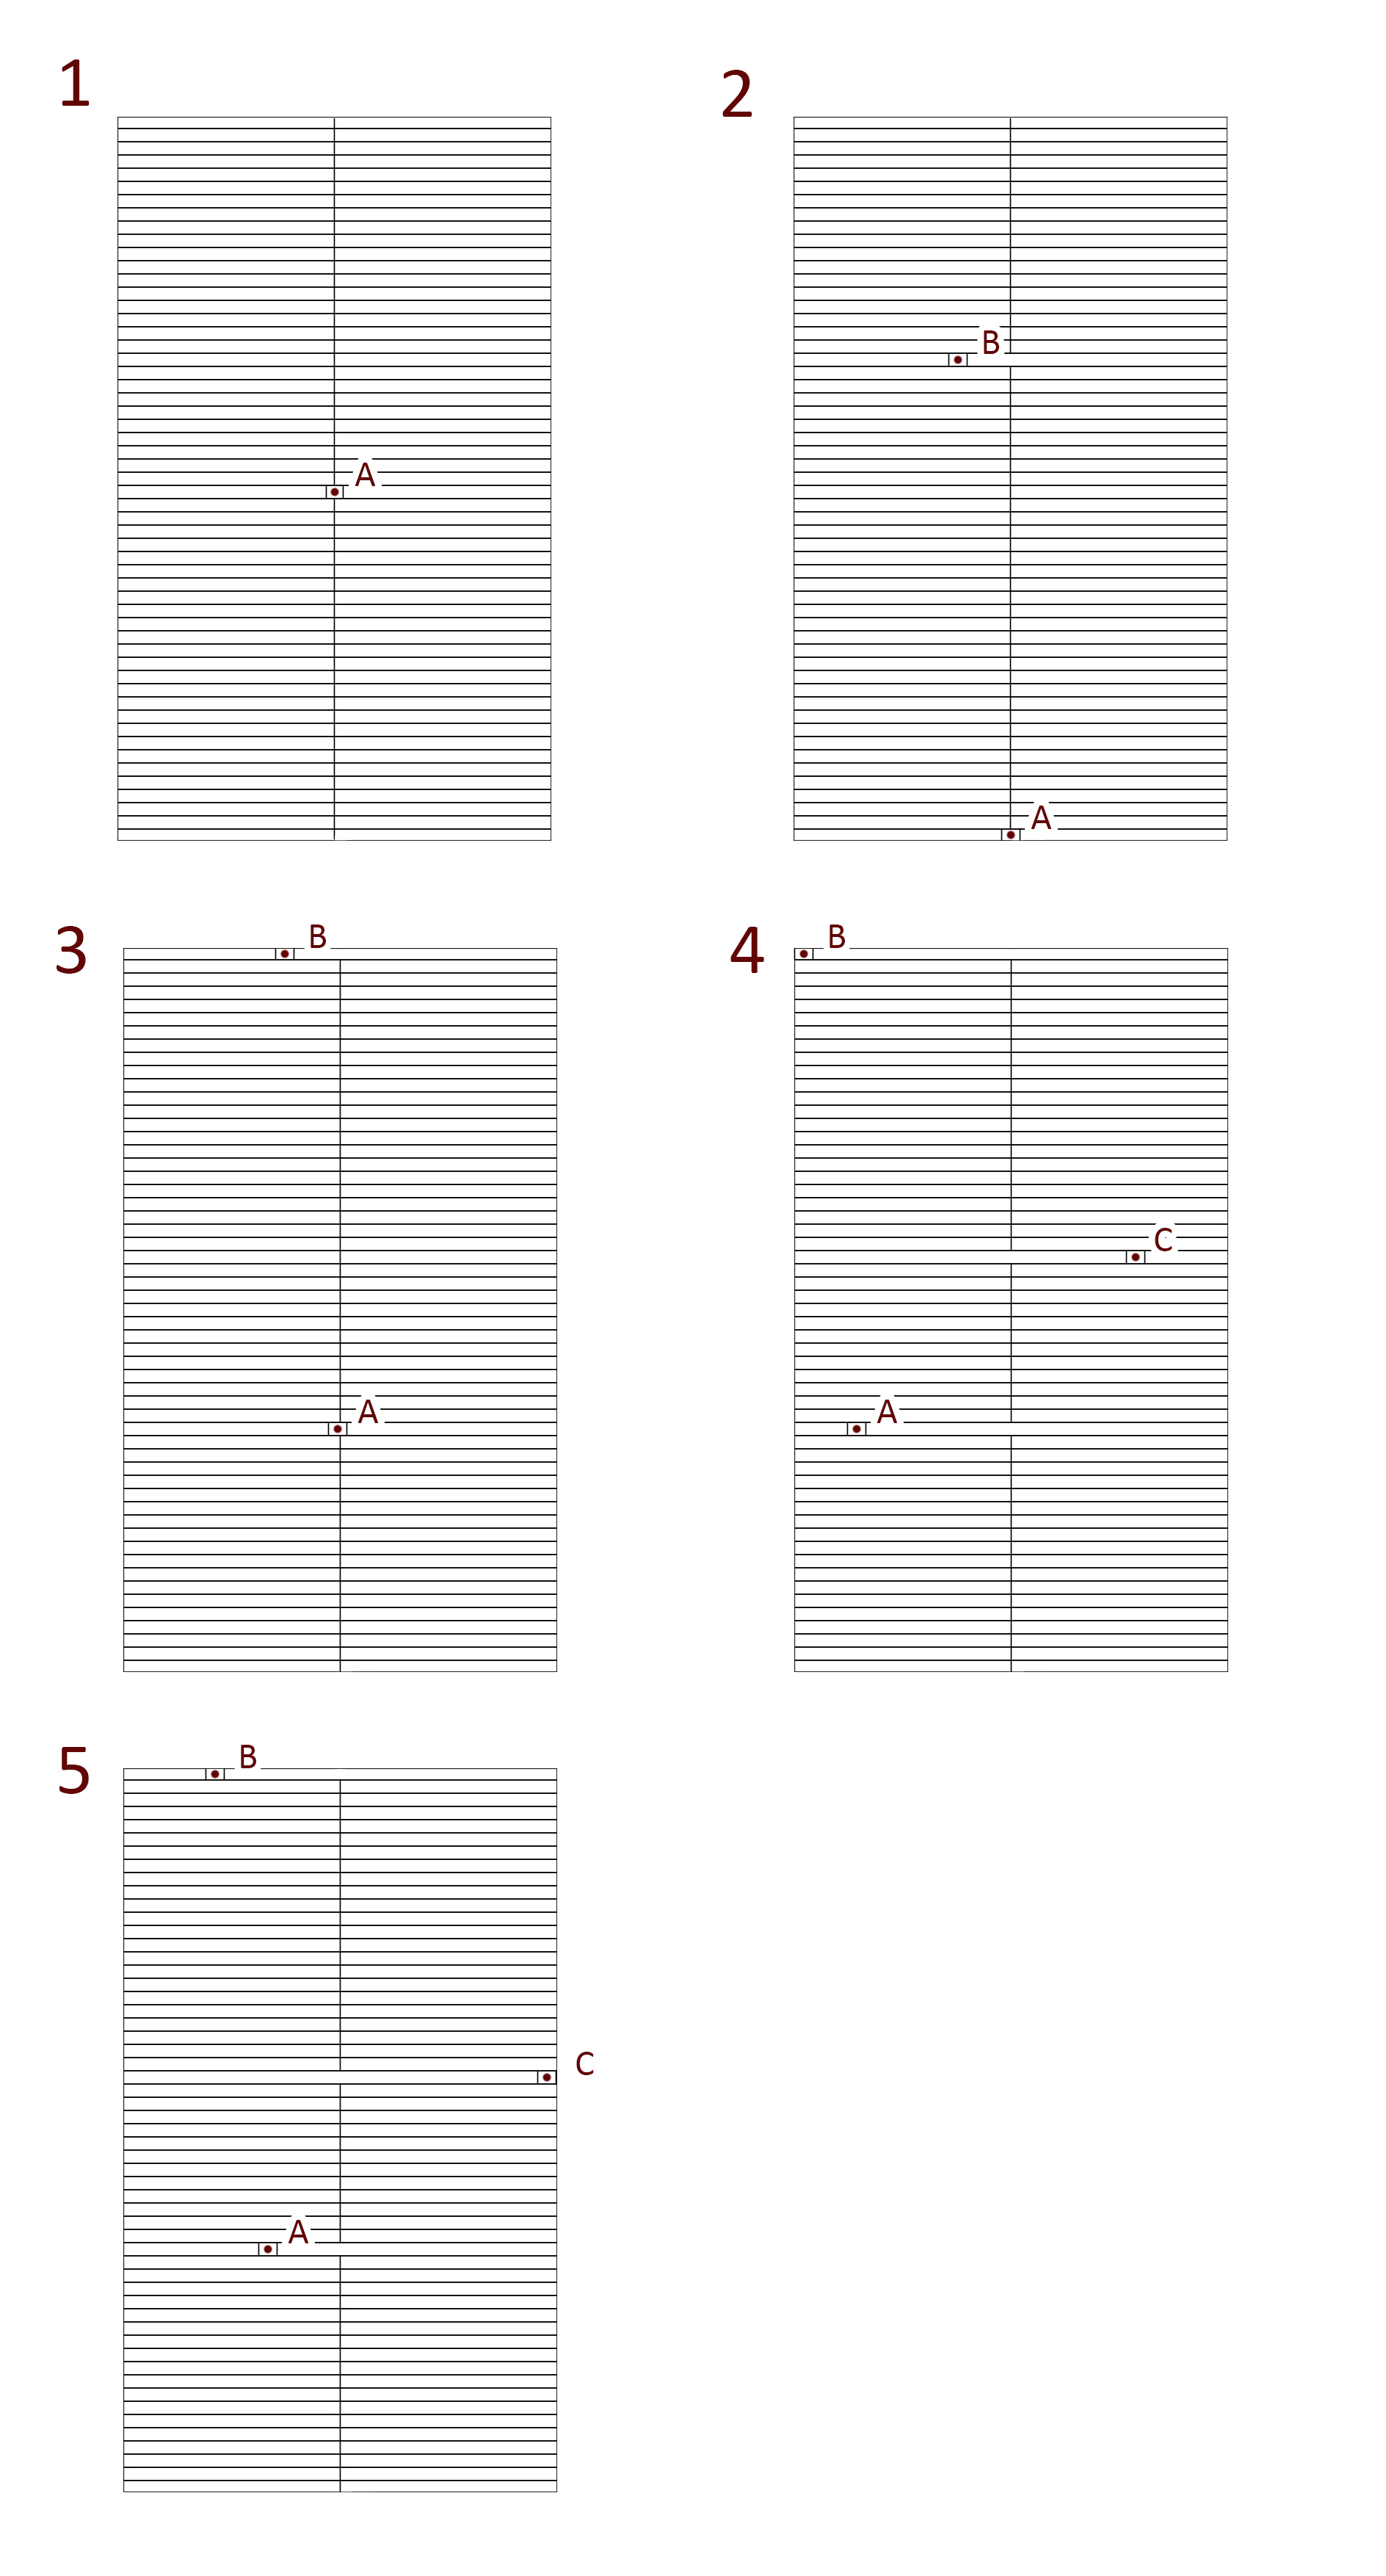
\includegraphics[width=0.7\linewidth]{CSU-algoritmo}
\caption{Movimientos de una CSU en el proceso de mejora}
\label{fig:mejora}
\end{figure}
%%%%%%%%%%%%%%%%%%%%%%%%%%%%%%%%%%%%%%%%%%%%%%%%%%%%%%%%%%%%%

La función \texttt{rellenar\_con\_puntos} del Algoritmo \ref{alg:const2} es la
que se encarga de analizar objeto por objeto si éste está dentro o no de un
apuntado, y en caso afirmativo, lo añade al mismo. 
Se considera que un punto está dentro de una CSU si:
\begin{itemize}
\item Se encuentra en el área abarcada por la CSU
\item Se sitúa sobre una barra que no tiene ningún objeto asociado a ella y 
\item El objeto cumple las restricciones físicas elegidas por el usuario, como puede ser que no
sobrepase el límite de distancia respecto al borde de la barra o que se
encuentre en la parte superior de la misma. 
\end{itemize}
Existen ocasiones en las que un
objeto no ajusta en una barra por un margen muy pequeño, bien porque la barra esté
ocupada ya por otro punto o porque esté en un rango no válido de la misma. 
En estas ocasiones, en lugar de descartar el objeto y buscar otro que sí ajuste, se ha hallado que
es preferible adaptar la CSU (siempre que ello sea posible, cumpliendo siempre con las
restricciones previamente definidas) para que éste entre en el apuntado.

\subsection{Fase 2} \label{subsec:fase2}
Una vez se tiene una solución al problema, es decir, un conjunto de apuntados
que ``cubren'' todos los objetos del problema, se intenta mejorar la solución eliminando o
reduciendo las colisiones entre apuntados. 
Diremos que un apuntado \textit{colisiona} con
otro cuando la intersección de las áreas cubiertas es no vacía.
Ello puede ocasionar que un objeto sea asociado a más de un apuntado.
Supongamos que se asocia con dos apuntados $A$ y $B$.
En este caso lo que
se intenta es crear un nuevo apuntado (CSU) $C$ con posición diferente a las
anteriores, que o bien las sustituya o bien consiga una mejora respecto a
alguna, es decir, $C$ mejor que $A$, $C$ mejor que $B$ o $C \equiv A \bigcup B$.
Esto se consigue iterando sobre el subconjunto de objetos son abarcados por $A$ y $B$
con un número mucho mayor de rotaciones de CSU. 
El Algoritmo \ref{alg:const3} presenta el esquema del algoritmo.

\begin{algorithm}[H]
$lista_{fin} \leftarrow \O$

$lista_{ini} =$ resultado

\While{(Mientras se mejore el resultado)} {

    $lista_{fin} =$ los que no colisionan con ninguno.

    \While{(queden objetos por cubrir)} {

        CSU $C \leftarrow$ primer apuntado $\in lista_{ini}$

        $subcto\_puntos = $ puntos de $C$

        Quitar $C$ de $lista_{ini}$

        \While{(queden CSUs $Q$ por mirar en $lista_{ini}$)} {

            \If{($Q$ colisiona con $C$)} {

                $subcto\_puntos += $ puntos de $Q$

                Quitar $Q$ de $lista_{ini}$

            }

        }

        \If{(colisión innecesaria)} {

            Obtener\_nuevos\_apuntados($subcto\_puntos$)

            \eIf{(consigue mejorar)} {$lista_{ini} +=$ nuevos apuntado } 
             {

                Introducir en $lista_{ini}$ los que se quitaron

                Poner en $lista_{fin}$ el apuntado $C$

             }

        }

    }

    $lista_{ini} = lista_{fin}$
}
\caption{Pseudo-código del algoritmo para reducir colisiones}
\label{alg:const3}
\end{algorithm}

Puesto que cada objeto puede tener una prioridad superior a la del resto (siendo
el 1 la mayor prioridad), se ha añadido también prioridad a los apuntados, de
modo que la prioridad del mismo la decide el objeto con mayor prioridad
contenido en dicha CSU. Una vez obtenidos los resultados, los apuntados son
ordenados por prioridades, situando primero los de mayor prioridad. 
En caso de que varios apuntados presenten la misma prioridad, se ordenarán según el número
de objetos que abarquen los mismos, colocando en primer lugar aquellos
apuntados cuyas barras estén completas.

En el Capítulo \ref{chap:aplication} se expone en detalle la implementación de todos
estos algoritmos y en qué punto del código de la aplicación se encuentran.

